\begin{table*}[t!]
\centering
\vspace{-0.03in}
\caption{Complexities of methods on novel view synthesis w/ $n$ input.
Prefill and rendering speed are measured on A100 with 48 512$\times$512 input images
% input images at 512$\times$512 resolution
(196K input tokens, 4K decoding tokens).}
\label{tab:attention_comparison}
\resizebox{\textwidth}{!}{%
\begin{tabular}{lccccll}
\toprule
 & \textbf{State Size} & \textbf{Prefill Compute} & \textbf{Decoding Compute} & \textbf{\# Params} & \textbf{Prefill speed} & \textbf{Rendering FPS} \\
\midrule
Full attention & $O(n)$ & $O(n^2)$ & $O(n)$ & 284M & 16.1 s & 2.3 FPS \\
Perceiver Attention & $O(1)$ & $O(n^2)$ & $O(1)$ & 287M & 16.8 s & 34.4 FPS \\
Ours & $O(1)$ & $O(n)$ & $O(1)$ & 312M & 1.4 s & 38.7 FPS \\
% \midrule
% \multicolumn{7}{l}{ \textit{Optimization based methods} } \\
% 3DGS~\cite{kerbl20233d}   & $\sim$60M        & –         & –        & -  & 10 mins & 100-500 FPS  \\
\bottomrule
\end{tabular}%
}
\vspace{-0.1in}
\end{table*}

\begin{figure}[t!]
    \vspace{-0.1in}
    \centering
    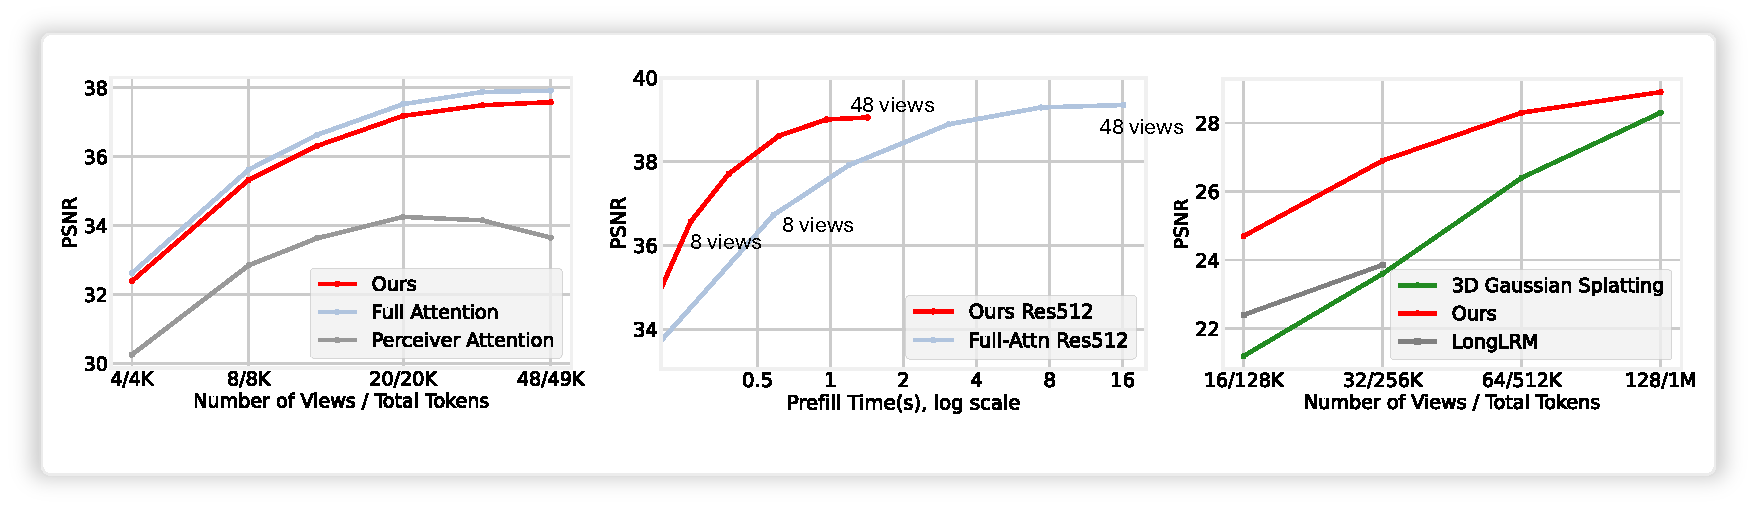
\includegraphics[width=\textwidth]{figures/figure_view_synthesis.pdf}
    \put(-345, 100){\capfontscriptsize GSO 256$\times$256}
    \put(-215, 100){\capfontscriptsize GSO 512$\times$512}
    \put(-100, 100){\capfontscriptsize DL3DV 960$\times$536}
    \put(-355,11){\capfont  \textbf{(a)} Object dataset }
    \put(-260,11){\capfont \textbf{(b)} Performance v.s. Prefill speed}
    \put(-130,11){\capfont \textbf{(c)} Scene dataset with 1M tokens}
    \vspace{-0.15in}
    \caption{\textbf{(a, b)} our method achieves quality comparable to full-attention models with significantly lower prefill latency,  and it clearly outperforms perceiver-attention baselines. \textbf{(c)} On the high resolution scene dataset, our approach surpasses LongLRM, limited to 32 views, and outperforms 3D Gaussian Splatting with sparse views, remaining competitive up to 128 input views (1M total tokens). }
    \vspace{-0.14in}
    \label{fig:view_syn_results}
\end{figure}
